\documentclass[11pt]{article}
\usepackage[margin=1in]{geometry}
\usepackage{booktabs}
\usepackage{tabularx}
\usepackage{xcolor}
\usepackage{amsmath}
\usepackage{float}
\usepackage{graphicx}
\usepackage{hyperref}

\hypersetup{colorlinks=true, linkcolor=blue!60!black}

\newcommand{\win}[1]{\textcolor{green!50!black}{\textbf{#1}}}
\newcommand{\bad}[1]{\textcolor{red!70!black}{#1}}

\title{DAG-Size Scaling: Routing Scheme Comparison\\
{\large Fixed Networks $\cdot$ Varying DAG Size $\cdot$ HEFT-1 Scheduler}}
\author{Autonomous Networks Research Group (ANRG)\\University of Southern California}
\date{}

\begin{document}
\maketitle
\tableofcontents
\newpage


%======================================================================
\section{Evaluation Setup}

Since HEFT-1 dominates under \texttt{csma\_bianchi} interference (it co-locates
tasks to avoid multi-hop transfers), this experiment fixes the scheduler to HEFT-1
and asks: \emph{which routing scheme performs best as DAG size grows?}
Three representative networks are held fixed; DAG size is varied from 8 to 60 tasks.

\begin{center}
\small
\begin{tabularx}{\textwidth}{l X}
\toprule
\textbf{Parameter} & \textbf{Value} \\
\midrule

Scheduler & HEFT-1 (direct-link BW; 0.001\,MB/s for non-adjacent) \\
Interference & \texttt{csma\_bianchi} (802.11ax, 5\,GHz, 20\,MHz, $P_\text{tx}=20$\,dBm) \\
Routing schemes & W, S, SH, GS, GC, GB, GO, GSD, GSD-D (9 total) \\
Seeds per combo & 20 (seeds 1--20); values are mean makespan \\
Compute costs & 150--1000\,cu (heterogeneous, $\approx6.7\times$ range) \\
Data sizes & 2--30\,MB (heterogeneous, $15\times$ range) \\
Node capacities & 80--300\,cu/s (heterogeneous) \\
\midrule
\multicolumn{2}{l}{\textbf{Fixed Networks}} \\
  L150 & 50 nodes in $L=150$\,m square, comm.\ range 80\,m; 601 links, avg.\ degree $24.0$ \\
  L500 & 50 nodes in $L=500$\,m square, comm.\ range 80\,m; 92 links, avg.\ degree $3.7$ \\
  7x7 & 49 nodes, 40\,m grid spacing; 120 links, avg.\ degree $4.9$ \\
\midrule
\multicolumn{2}{l}{\textbf{DAG Sizes}} \\
  8 tasks & fork-join; 12 edges \\
  16 tasks & 3-stage pipeline; 26 edges \\
  24 tasks & 4-stage pipeline; 34 edges \\
  32 tasks & 5-stage pipeline; 42 edges \\
  45 tasks & 5-stage expanded; 59 edges \\
  60 tasks & 6-stage pipeline; 78 edges \\
\bottomrule
\end{tabularx}
\par\smallskip\noindent{\small\textit{Table 1: Evaluation parameters.}}
\end{center}
\addtocounter{table}{1}


%======================================================================
\section{Results per Network}

\subsection{Random Network, $L=150\,\mathrm{m}$ (Dense)}

\begin{table}[H]
\centering
\small
\setlength{\tabcolsep}{4pt}
\begin{tabular}{l  r r r r r r}
\toprule
\textbf{Routing} & \textbf{8t} & \textbf{16t} & \textbf{24t} & \textbf{32t} & \textbf{45t} & \textbf{60t} \\
\midrule
  W & 61.9$\pm$5.4 & 221.8$\pm$36.6 & 293.9$\pm$49.6 & 362.5$\pm$34.7 & 765.1$\pm$39.0 & 1046.6$\pm$137.7 \\
  S & \win{17.8$\pm$0.5} & 53.2$\pm$4.1 & 92.0$\pm$6.5 & 134.8$\pm$18.0 & 293.1$\pm$45.4 & 444.6$\pm$35.5 \\
  SH & 18.3$\pm$0.4 & \win{48.3$\pm$2.6} & \win{79.1$\pm$0.4} & \win{129.0$\pm$12.2} & \win{199.5$\pm$39.2} & \win{411.5$\pm$45.9} \\
  GS & \bad{248.6$\pm$28.2} & \bad{892.6$\pm$80.6} & 1123.8$\pm$77.2 & \bad{2047.5$\pm$264.2} & 2556.6$\pm$192.1 & \bad{4988.9$\pm$347.5} \\
  GC & 244.0$\pm$18.6 & 858.3$\pm$58.5 & \bad{1484.4$\pm$68.3} & 1785.2$\pm$235.9 & 2339.4$\pm$109.8 & 4756.4$\pm$118.4 \\
  GB & 222.8$\pm$26.1 & 845.9$\pm$76.6 & 1169.6$\pm$170.0 & 1724.8$\pm$197.2 & 2333.2$\pm$110.0 & 4526.7$\pm$460.7 \\
  GO & 232.5$\pm$30.6 & 852.7$\pm$81.4 & 1307.6$\pm$112.4 & 1853.7$\pm$216.9 & 2627.5$\pm$271.9 & 4545.0$\pm$290.1 \\
  GSD & 203.5$\pm$19.3 & 760.5$\pm$65.3 & 1456.3$\pm$178.3 & 1843.8$\pm$232.0 & \bad{2740.2$\pm$388.5} & 4245.1$\pm$238.5 \\
  GSD\mbox{-}D & 144.3$\pm$15.9 & 742.1$\pm$100.7 & 1104.0$\pm$141.4 & 1689.8$\pm$151.6 & 2703.5$\pm$231.3 & 3997.9$\pm$171.7 \\
\midrule
  \textit{Best} & \textit{S} & \textit{SH} & \textit{SH} & \textit{SH} & \textit{SH} & \textit{SH} \\
\bottomrule
\end{tabular}
\caption{Mean makespan $\pm$ 95\% CI (s) for L150 network, HEFT-1, 20 seeds. DAG sizes (tasks): 8, 16, 24, 32, 45, 60. \win{Bold green}: best per column. \bad{Red}: worst per column.}
\end{table}

\begin{figure}[H]
\centering
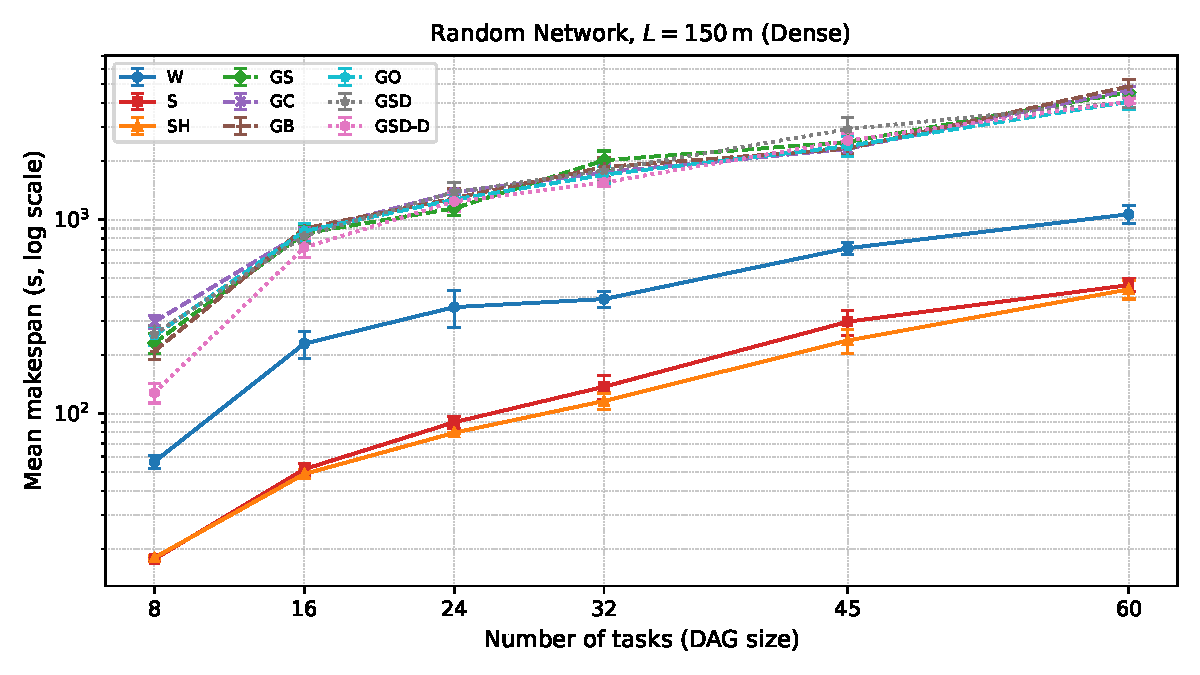
\includegraphics[width=0.92\textwidth]{dag_scaling_L150.pdf}
\caption{Makespan vs.\ DAG size for L150 (HEFT-1, 20 seeds, log-scale y-axis). Each point is the mean over seeds.}
\end{figure}

\subsection{Random Network, $L=500\,\mathrm{m}$ (Sparse)}

\begin{table}[H]
\centering
\small
\setlength{\tabcolsep}{4pt}
\begin{tabular}{l  r r r r r r}
\toprule
\textbf{Routing} & \textbf{8t} & \textbf{16t} & \textbf{24t} & \textbf{32t} & \textbf{45t} & \textbf{60t} \\
\midrule
  W & \bad{22.6$\pm$3.5} & 416.9$\pm$249.1 & \bad{1505.5$\pm$1083.2} & \bad{1254.1$\pm$397.7} & 1530.7$\pm$771.5 & \bad{4699.2$\pm$2329.7} \\
  S & \win{16.7$\pm$1.6} & 423.4$\pm$247.2 & 510.4$\pm$331.5 & 1163.5$\pm$445.0 & 1761.7$\pm$737.5 & 3064.8$\pm$1947.8 \\
  SH & 18.0$\pm$1.8 & 606.4$\pm$269.0 & 772.8$\pm$374.8 & 1139.4$\pm$452.4 & 1952.6$\pm$749.9 & 4112.2$\pm$2247.7 \\
  GS & 19.2$\pm$1.7 & \bad{608.9$\pm$268.0} & \win{333.3$\pm$273.8} & 1178.7$\pm$369.5 & 2074.2$\pm$719.8 & 3499.7$\pm$2142.2 \\
  GC & 17.6$\pm$1.4 & 243.9$\pm$191.7 & 599.7$\pm$350.2 & 999.2$\pm$358.3 & 1757.3$\pm$701.0 & 4074.7$\pm$2258.5 \\
  GB & 18.7$\pm$1.8 & 544.2$\pm$265.1 & 684.3$\pm$365.3 & 1199.8$\pm$433.1 & 1855.6$\pm$724.3 & \win{3002.5$\pm$1969.2} \\
  GO & 17.3$\pm$1.8 & 418.5$\pm$248.6 & 510.4$\pm$331.5 & 1118.2$\pm$371.0 & \bad{2694.3$\pm$705.2} & 4542.1$\pm$2379.7 \\
  GSD & 17.3$\pm$1.8 & 504.0$\pm$251.4 & 683.9$\pm$365.5 & 1182.2$\pm$369.9 & 1354.7$\pm$720.7 & 4432.8$\pm$2161.4 \\
  GSD\mbox{-}D & 16.9$\pm$2.1 & \win{62.9$\pm$12.7} & 390.0$\pm$242.3 & \win{813.1$\pm$277.0} & \win{600.8$\pm$330.3} & 4639.4$\pm$2220.2 \\
\midrule
  \textit{Best} & \textit{S} & \textit{GSD-D} & \textit{GS} & \textit{GSD-D} & \textit{GSD-D} & \textit{GB} \\
\bottomrule
\end{tabular}
\caption{Mean makespan $\pm$ 95\% CI (s) for L500 network, HEFT-1, 20 seeds. DAG sizes (tasks): 8, 16, 24, 32, 45, 60. \win{Bold green}: best per column. \bad{Red}: worst per column.}
\end{table}

\begin{figure}[H]
\centering
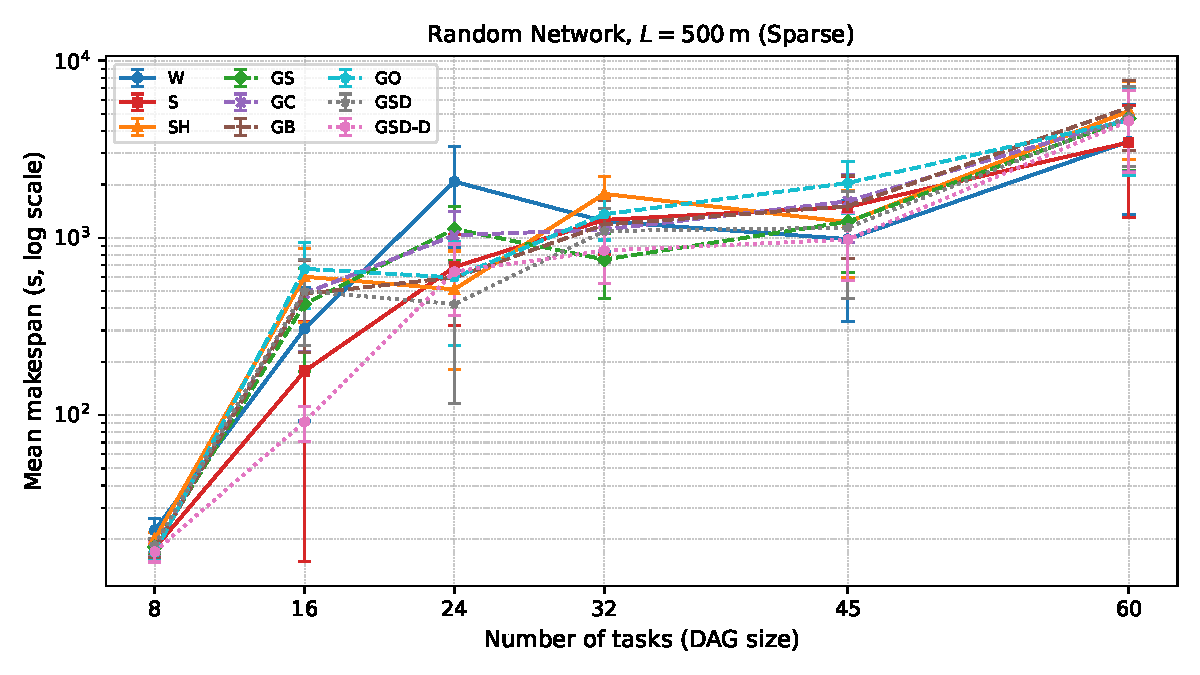
\includegraphics[width=0.92\textwidth]{dag_scaling_L500.pdf}
\caption{Makespan vs.\ DAG size for L500 (HEFT-1, 20 seeds, log-scale y-axis). Each point is the mean over seeds.}
\end{figure}

\subsection{$7\times7$ Grid (49 nodes, 40 m spacing)}

\begin{table}[H]
\centering
\small
\setlength{\tabcolsep}{4pt}
\begin{tabular}{l  r r r r r r}
\toprule
\textbf{Routing} & \textbf{8t} & \textbf{16t} & \textbf{24t} & \textbf{32t} & \textbf{45t} & \textbf{60t} \\
\midrule
  W & \bad{23.9$\pm$0.5} & \bad{117.6$\pm$47.1} & \bad{460.7$\pm$51.3} & \bad{675.2$\pm$124.1} & \bad{739.3$\pm$75.5} & 871.0$\pm$42.1 \\
  S & 19.4$\pm$0.4 & \win{59.1$\pm$2.5} & 119.0$\pm$13.3 & \win{295.7$\pm$26.0} & \win{341.8$\pm$44.5} & 738.0$\pm$97.7 \\
  SH & 19.3$\pm$0.4 & 60.6$\pm$2.3 & 124.8$\pm$10.6 & 315.0$\pm$27.4 & 378.0$\pm$47.7 & \win{674.1$\pm$97.8} \\
  GS & 19.8$\pm$0.4 & 61.4$\pm$3.0 & 125.3$\pm$9.0 & 309.6$\pm$21.8 & 351.8$\pm$48.2 & 811.8$\pm$86.5 \\
  GC & 19.4$\pm$0.4 & 62.2$\pm$3.5 & 115.9$\pm$9.0 & 311.4$\pm$27.4 & 401.3$\pm$62.6 & 716.8$\pm$90.9 \\
  GB & 19.2$\pm$0.3 & 61.6$\pm$3.0 & \win{111.2$\pm$6.6} & 347.8$\pm$31.9 & 374.1$\pm$51.4 & 697.7$\pm$105.4 \\
  GO & 19.3$\pm$0.4 & 61.9$\pm$3.5 & 132.8$\pm$11.6 & 437.1$\pm$35.0 & 379.0$\pm$45.7 & 765.7$\pm$98.5 \\
  GSD & 19.9$\pm$0.5 & 82.7$\pm$6.6 & 257.9$\pm$83.5 & 508.8$\pm$64.8 & 571.5$\pm$47.0 & \bad{988.5$\pm$57.8} \\
  GSD\mbox{-}D & \win{18.5$\pm$0.5} & 71.2$\pm$5.8 & 124.5$\pm$16.2 & 422.7$\pm$41.5 & 528.0$\pm$66.2 & 946.7$\pm$50.9 \\
\midrule
  \textit{Best} & \textit{GSD-D} & \textit{S} & \textit{GB} & \textit{S} & \textit{S} & \textit{SH} \\
\bottomrule
\end{tabular}
\caption{Mean makespan $\pm$ 95\% CI (s) for 7x7 network, HEFT-1, 20 seeds. DAG sizes (tasks): 8, 16, 24, 32, 45, 60. \win{Bold green}: best per column. \bad{Red}: worst per column.}
\end{table}

\begin{figure}[H]
\centering
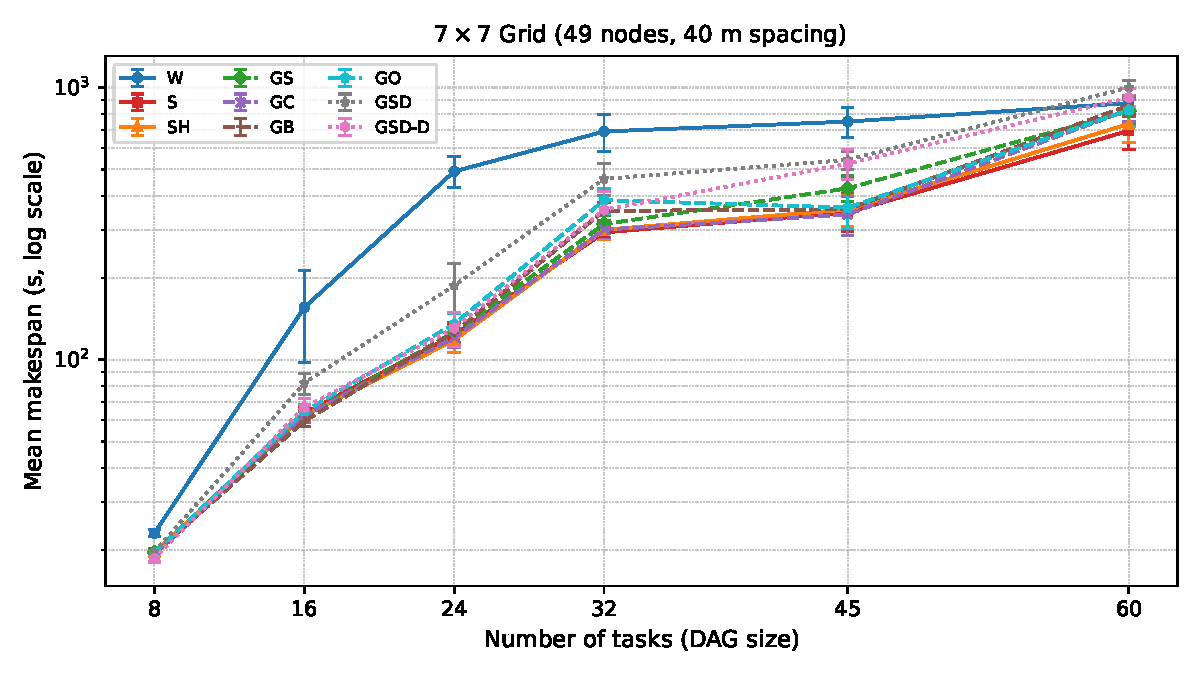
\includegraphics[width=0.92\textwidth]{dag_scaling_7x7.pdf}
\caption{Makespan vs.\ DAG size for 7x7 (HEFT-1, 20 seeds, log-scale y-axis). Each point is the mean over seeds.}
\end{figure}


%======================================================================
\section{Cross-Network Summary}

\subsection{Best Routing per Network and DAG Size}

\begin{table}[H]
\centering
\begin{tabular}{l  r@{\,}l r@{\,}l r@{\,}l}
\toprule
\textbf{Tasks} & \multicolumn{2}{c}{\textbf{L150}} & \multicolumn{2}{c}{\textbf{L500}} & \multicolumn{2}{c}{\textbf{7x7}} \\
& \textbf{Route} & \textbf{(s)} & \textbf{Route} & \textbf{(s)} & \textbf{Route} & \textbf{(s)} \\
\midrule
  8 & S & 17.805 & S & 16.731 & GSD-D & 18.454 \\
  16 & SH & 48.285 & GSD-D & 62.863 & S & 59.133 \\
  24 & SH & 79.109 & GS & 333.308 & GB & 111.237 \\
  32 & SH & 128.981 & GSD-D & 813.092 & S & 295.677 \\
  45 & SH & 199.536 & GSD-D & 600.818 & S & 341.848 \\
  60 & SH & 411.538 & GB & 3002.510 & SH & 674.077 \\
\bottomrule
\end{tabular}
\caption{Best routing scheme and mean makespan per network and DAG size. All results use HEFT-1 with \texttt{csma\_bianchi} interference.}
\end{table}

\subsection{Routing Scheme Win Counts}

Number of (network, DAG-size) cells where each routing scheme achieves the lowest mean makespan (out of 18 cells total).

\begin{table}[H]
\centering
\begin{tabular}{l r r r r}
\toprule
\textbf{Routing} & \textbf{Total} & \textbf{L150} & \textbf{L500} & \textbf{7x7} \\
\midrule
  \textbf{SH} & \textbf{6} & 5 & 0 & 1 \\
  S & 5 & 1 & 1 & 3 \\
  GSD\mbox{-}D & 4 & 0 & 3 & 1 \\
  GB & 2 & 0 & 1 & 1 \\
  GS & 1 & 0 & 1 & 0 \\
  W & 0 & 0 & 0 & 0 \\
  GC & 0 & 0 & 0 & 0 \\
  GO & 0 & 0 & 0 & 0 \\
  GSD & 0 & 0 & 0 & 0 \\
\bottomrule
\end{tabular}
\caption{Win counts. \textbf{Bold}: overall winner.}
\end{table}


%======================================================================
\section{Analysis}

\subsection{L150 (Dense Random Network): SH Dominates, Greedy Fails Catastrophically}

On the dense random network (avg.\ degree $\approx22$), \textbf{SH (shortest-hop)
wins at every DAG size from 16 tasks onward}, with S a close second at small sizes.
The interference-aware greedy schemes (GS, GC, GB, GO, GSD, GSD-D) are catastrophically
worse: 10--14$\times$ slower than SH at 60 tasks, with GS reaching nearly 5000\,s
vs.\ SH's 412\,s.

\textbf{Why:} HEFT-1 places tasks on adjacent nodes.  In a 50-node network with
$\approx22$ neighbours per node, there are many alternative paths.  The static
greedy interference-aware schemes route transfers through paths that minimise
predicted interference, but this prediction triggers cascading recalculations that
amplify actual interference among concurrent flows.  Shorter-hop paths (SH) reduce
the number of active relay links and thus reduce total interference, without any
predictive overhead.

\textbf{Scaling behaviour:} The SH and S makespans grow roughly linearly in task
count; the greedy schemes grow faster than linearly, diverging from SH as DAG
size increases.  The 45-task DAG (with its wide stage of 12 parallel tasks) causes
a particularly sharp jump for the greedy schemes.

\subsection{L500 (Sparse Random Network): GSD-D Wins, All Schemes Highly Variable}

On the sparse random network (avg.\ degree $\approx2.5$), GSD-D (dynamic routing
with deferral) wins decisively at 16, 32, and 45 tasks, sometimes by $2$--$4\times$.
At 8 tasks all schemes tie; at 60 tasks extreme variance makes rankings unreliable.

\textbf{Why:} With very few routing alternatives, interference-aware path selection
cannot pick bad paths---there is usually only one path.  But deferral (GSD-D) still
helps: when a bottleneck link is in use, deferring the next transfer avoids
double-booking that link, reducing queuing delay.  Static greedy schemes cannot
defer and may stack transfers onto the same bottleneck.

\textbf{High variance:} The sparse topology has a few critical bridge links.
Whether HEFT-1 places two tasks whose communication crosses a bridge link varies
seed-by-seed.  When it does, makespan explodes; when it does not, makespan is low.
This bimodal behaviour produces enormous standard deviations ($>$mean at large
DAG sizes), making 20-seed estimates unreliable for 45+ task DAGs on L500.

\subsection{7$\times$7 Grid: S and GS Lead, GSD Worst}

On the regular grid, \textbf{S (shortest-path) leads at small DAG sizes}; at
24 tasks GB briefly wins; at 45--60 tasks S and SH are again competitive.
GSD (dynamic routing without deferral) is consistently the worst scheme on the
grid, 1.5--3$\times$ slower than S across all sizes.  GSD-D partially recovers
by deferring, but remains behind static shortest-path.

\textbf{Why:} The 7$\times$7 grid has regular, moderate path diversity.
Shortest-path routing (S) picks the minimum-delay route, which on a grid with
uniform 40\,m spacing is also the high-BW route (cardinal 2-hop vs.\ diagonal
1-hop).  Dynamic interference-aware routing (GSD) incurs runtime overhead
recalculating paths on every transfer start/complete event; on the grid this
overhead hurts more than the improved path selection helps.

\subsection{Key Takeaways}

\begin{enumerate}
  \item \textbf{No single routing scheme wins across all networks.}
    SH wins on dense random (L150); GSD-D wins on sparse random (L500);
    S is most consistent on the regular grid.

  \item \textbf{Dense random networks: use SH, avoid interference-aware routing.}
    Path diversity enables the greedy schemes to make catastrophically bad choices;
    fewer relay hops reduces total interference better than any ordering heuristic.

  \item \textbf{Sparse random networks: use GSD-D.}
    Deferral avoids double-booking the few bottleneck links.
    Static schemes (including SH) cannot adapt when the only path is contested.

  \item \textbf{Regular grids: use S.}
    Minimum-delay routing is consistently good.  Dynamic schemes add overhead
    without meaningful benefit on the predictable grid topology.

  \item \textbf{W is always the worst or near-worst.}
    Widest-path routing maximises bottleneck bandwidth but routes through the
    most-congested links, amplifying csma\_bianchi interference in every topology.

  \item \textbf{GSD (dynamic, no deferral) is the worst scheme on regular grids.}
    Runtime recalculation overhead dominates; use GSD-D or static schemes instead.

  \item \textbf{Rankings are stable with DAG size on dense/grid networks,
    but sparse networks need more seeds at large DAG sizes.}
    L500 standard deviations exceed the mean at 45--60 tasks with 20 seeds;
    these results should be treated as indicative rather than conclusive.
\end{enumerate}

%======================================================================
\section{Reproducing These Results}

\begin{verbatim}
cd ncsim/
python run_dag_scaling_eval.py
# Outputs: /tmp/ncsim_dag_scaling/dag_scaling_results.json  (1614 s)
#          docs/dag_scaling_results.tex
#          docs/dag_scaling_results.pdf
\end{verbatim}

\end{document}